\documentclass[a4paper,12pt]{article}

% Paquetes necesarios
\usepackage[utf8]{inputenc}     % Codificación de caracteres
\usepackage[spanish]{babel}     % Idioma del documento
\usepackage{amsmath, amssymb}   % Paquetes para símbolos y ecuaciones matemáticas
\usepackage{graphicx}           % Para insertar imágenes
\usepackage{caption}            % Para leyendas
\usepackage{subcaption}         % Para subfiguras
\usepackage{geometry}           % Control de márgenes
\usepackage{hyperref}           % Enlaces dentro del documento
\geometry{top=2cm, bottom=2cm, left=2cm, right=2cm}

% Datos del documento
\title{Trabajo Práctico 1}
\author{Alejo Ordoñez - 108397}
\date{Jueves 26 de Septiembre, 2024}

\begin{document}

\maketitle

\newpage
\tableofcontents


\newpage
\section{Introducción}

En este informe se presentan varios resultados obtenidos empíricamente a partir del entrenamiento de una red de Hopfield.\textit{}

\section{Red de Hopfield}
Vamos a entrenar un modelo de Hopfield con un conjunto de 6 imágenes. Primero vamos a elegir un subconjunto de las mismas para ver si puede aprenderlas, luego vamos a corromper esas imágenes para ver si aún así logra distinguirlas y por último vamos a intentar enseñárselas todas.

\begin{figure}[h]
    \centering
    \includegraphics[width=0.5\textwidth]{imágenes/figura1.png}
    \caption{Conjunto completo de imágenes originales utilizadas para el entrenamiento.}
    \label{fig:figura1}
\end{figure}

Una red de Hopfield es un modelo de memoria asociativa que usa la regla de Hebb para todos los pares $ij$ posibles, con unidades binarias y actualización asíncrona.

Regla de Hebb: $w_{ij} = \frac{1}{N} \sum_{\mu=1}^{p} \xi_{i}^{\mu} \xi_{j}^{\mu}$.

Para entrenar la red, se uniformiza el tamaño de las imágenes. En este caso decicí tomar como estándar las dimensiones de la imágen más grande y colocar aquellas que estuvieran por debajo sobre un fondo blanco de ese tamaño: 50 x 60.

La red de Hopfield, es en el notebook, una clase con métodos entrenar y recuperar. El entrenamiento consiste en asignar a los pesos la suma del producto de los patrones con sigo mismos, asegurando el 0 en la diagonal, pues las unidades no deben hacer sinpasis consigo mismas en este modelo.

\subsection{Verifación del aprendizaje}
Para verificar si la red aprendió o no las imágenes enseñadas, intentamos recuperarlas sin ninguna modificación. Se entrena primero el modelo con tres de las imágenes de la ~\ref{fig:figura1}. El resultado era el esperado, la red converge en las imágenes originales.

\begin{figure}[h]
    \centering
    \includegraphics[width=0.5\textwidth]{imágenes/figura2.png}
    \caption{Subconjunto de imágenes utilizadas para el primer entrenamiento.}
    \label{fig:figura2}
\end{figure}

\begin{figure}[h]
    \centering
    \includegraphics[width=0.5\textwidth]{imágenes/figura3.png}
    \caption{Imágenes recuperadas.}
    \label{fig:figura3}
\end{figure}

\subsection{Evaluación de versiones alteradas de las imágenes}
Para probar qué tan bien funciona la red, se distorsionan las imágenes que se intentan recuperar, con el objetivo de obtener las imágenes originales con las cuáles el modelo fue entrenado.

Primeramente se les agrega ruido a cada una de las imágenes. Esto se hace invirtiendo $(\text{nivel}*\text{tamaño de la imagen})$ píxeles. En este caso, se invirtieron la mitad de los píxeles. Al intentar recuperar las imágenes, la red las recordó correctamente.

\begin{figure}[h]
    \centering
    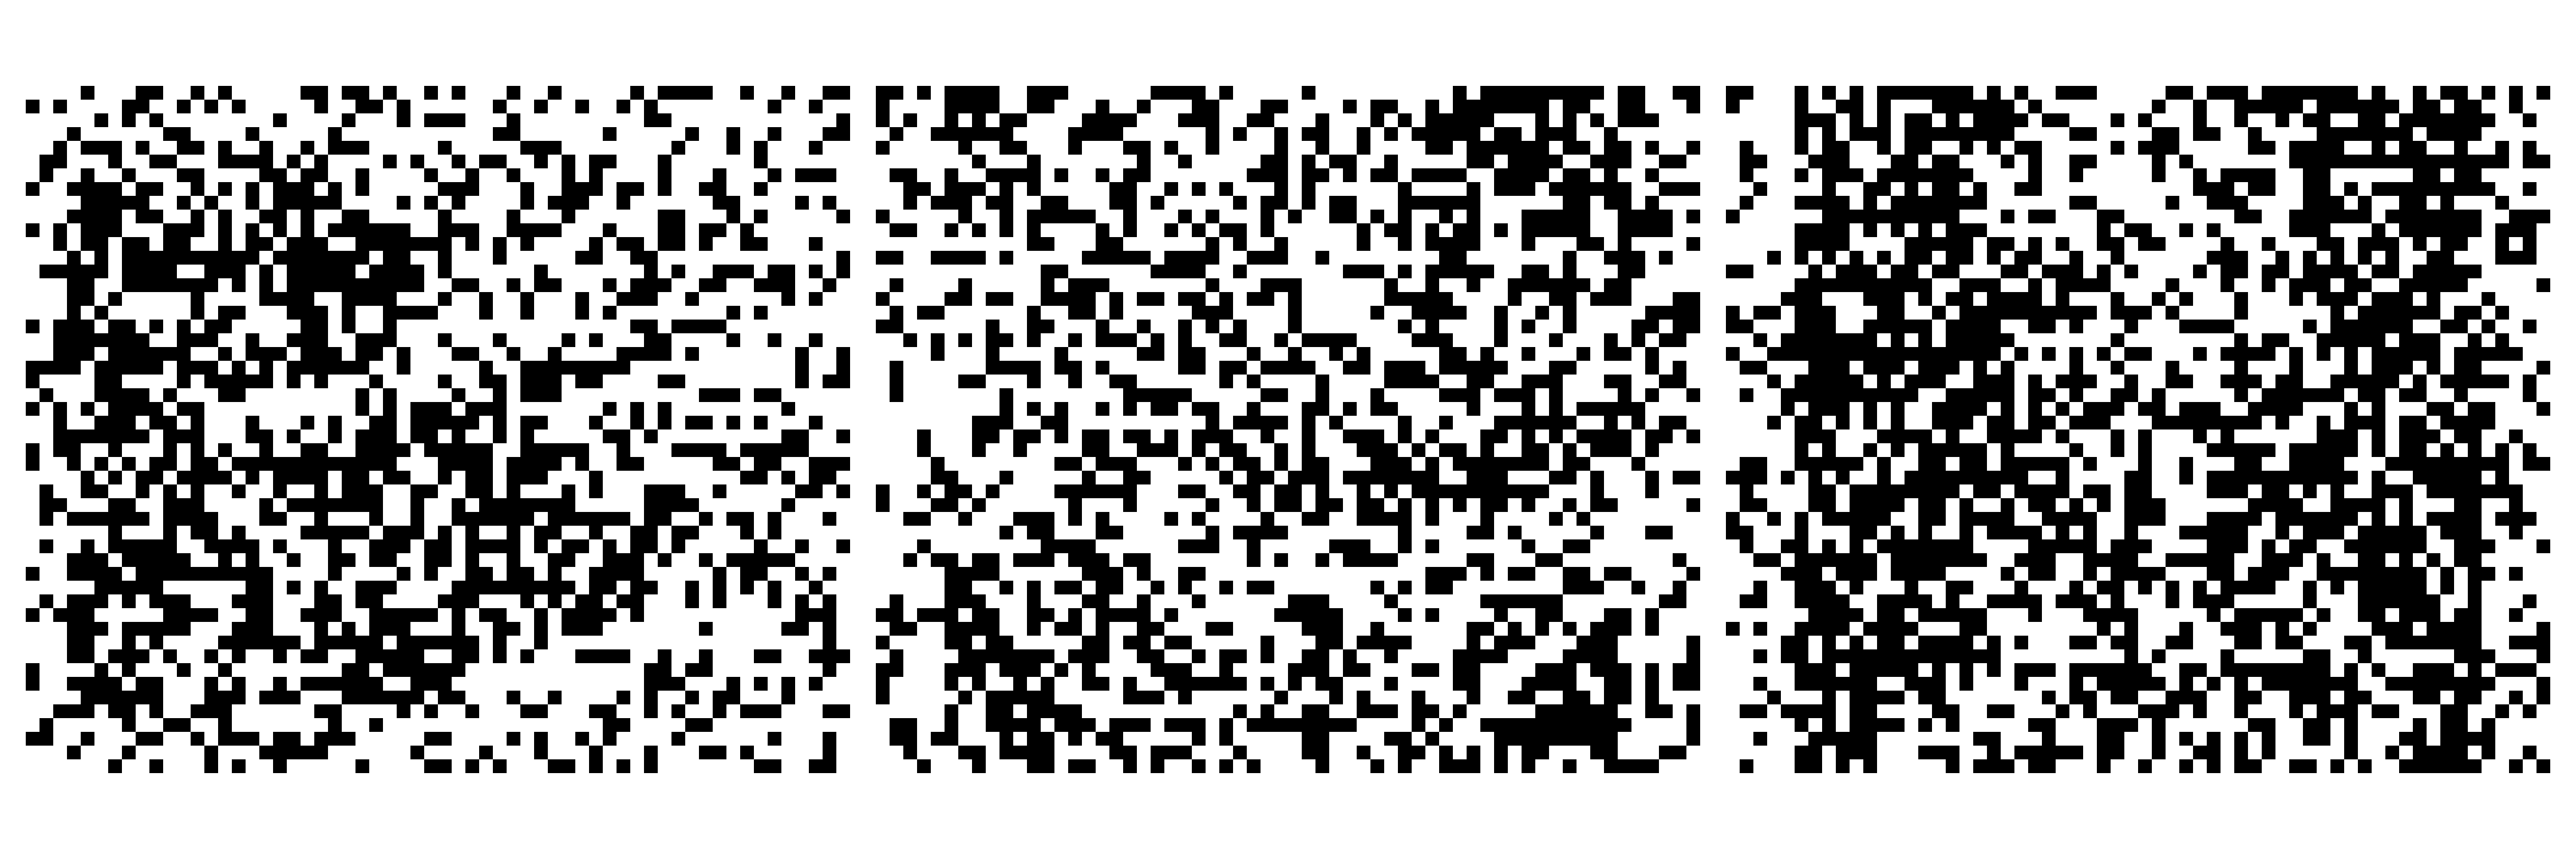
\includegraphics[width=0.5\textwidth]{imágenes/figura4.png}
    \caption{Imágenes con ruido.}
    \label{fig:figura4}
\end{figure}

\begin{figure}[h]
    \centering
    \includegraphics[width=0.5\textwidth]{imágenes/figura5.png}
    \caption{Imágenes recuperadas.}
    \label{fig:figura5}
\end{figure}

Nuevamente, corrompemos las imágenes, ésta vez eliminando cuadrados de tamaño $(text{nivel}*text{tamaño de la imagen})$ posicionados aleatoriamente. Y otra vez la red las recupera correctamente.

\begin{figure}[h]
    \centering
    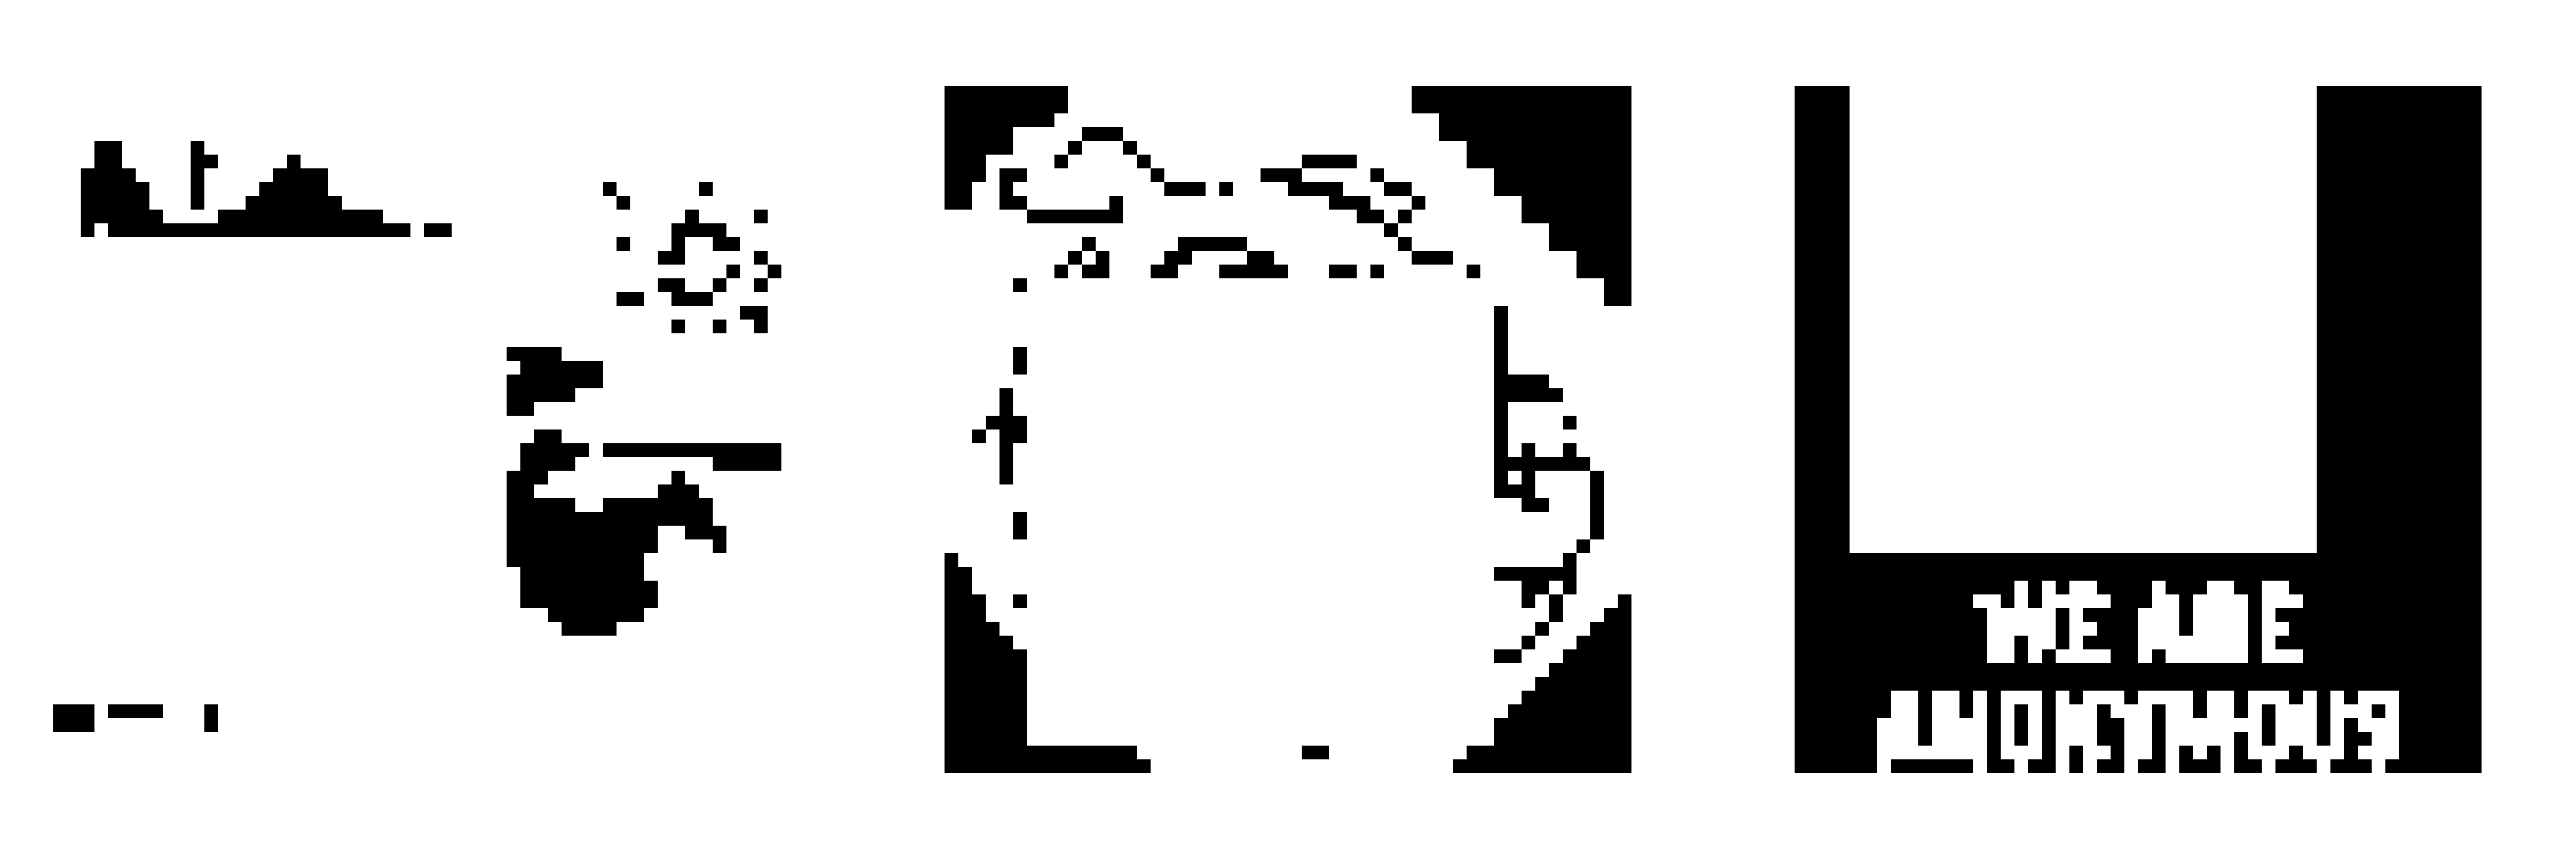
\includegraphics[width=0.5\textwidth]{imágenes/figura6.png}
    \caption{Imágenes con cuadrados removidos.}
    \label{fig:figura6}
\end{figure}

\begin{figure}[h]
    \centering
    \includegraphics[width=0.5\textwidth]{imágenes/figura7.png}
    \caption{Imágenes recuperadas.}
    \label{fig:figura7}
\end{figure}

Rotamos las imágenes $180^{\circ}$. Esta vez la red se equivoca, y confunde la primera con la segunda.

\begin{figure}[h]
    \centering
    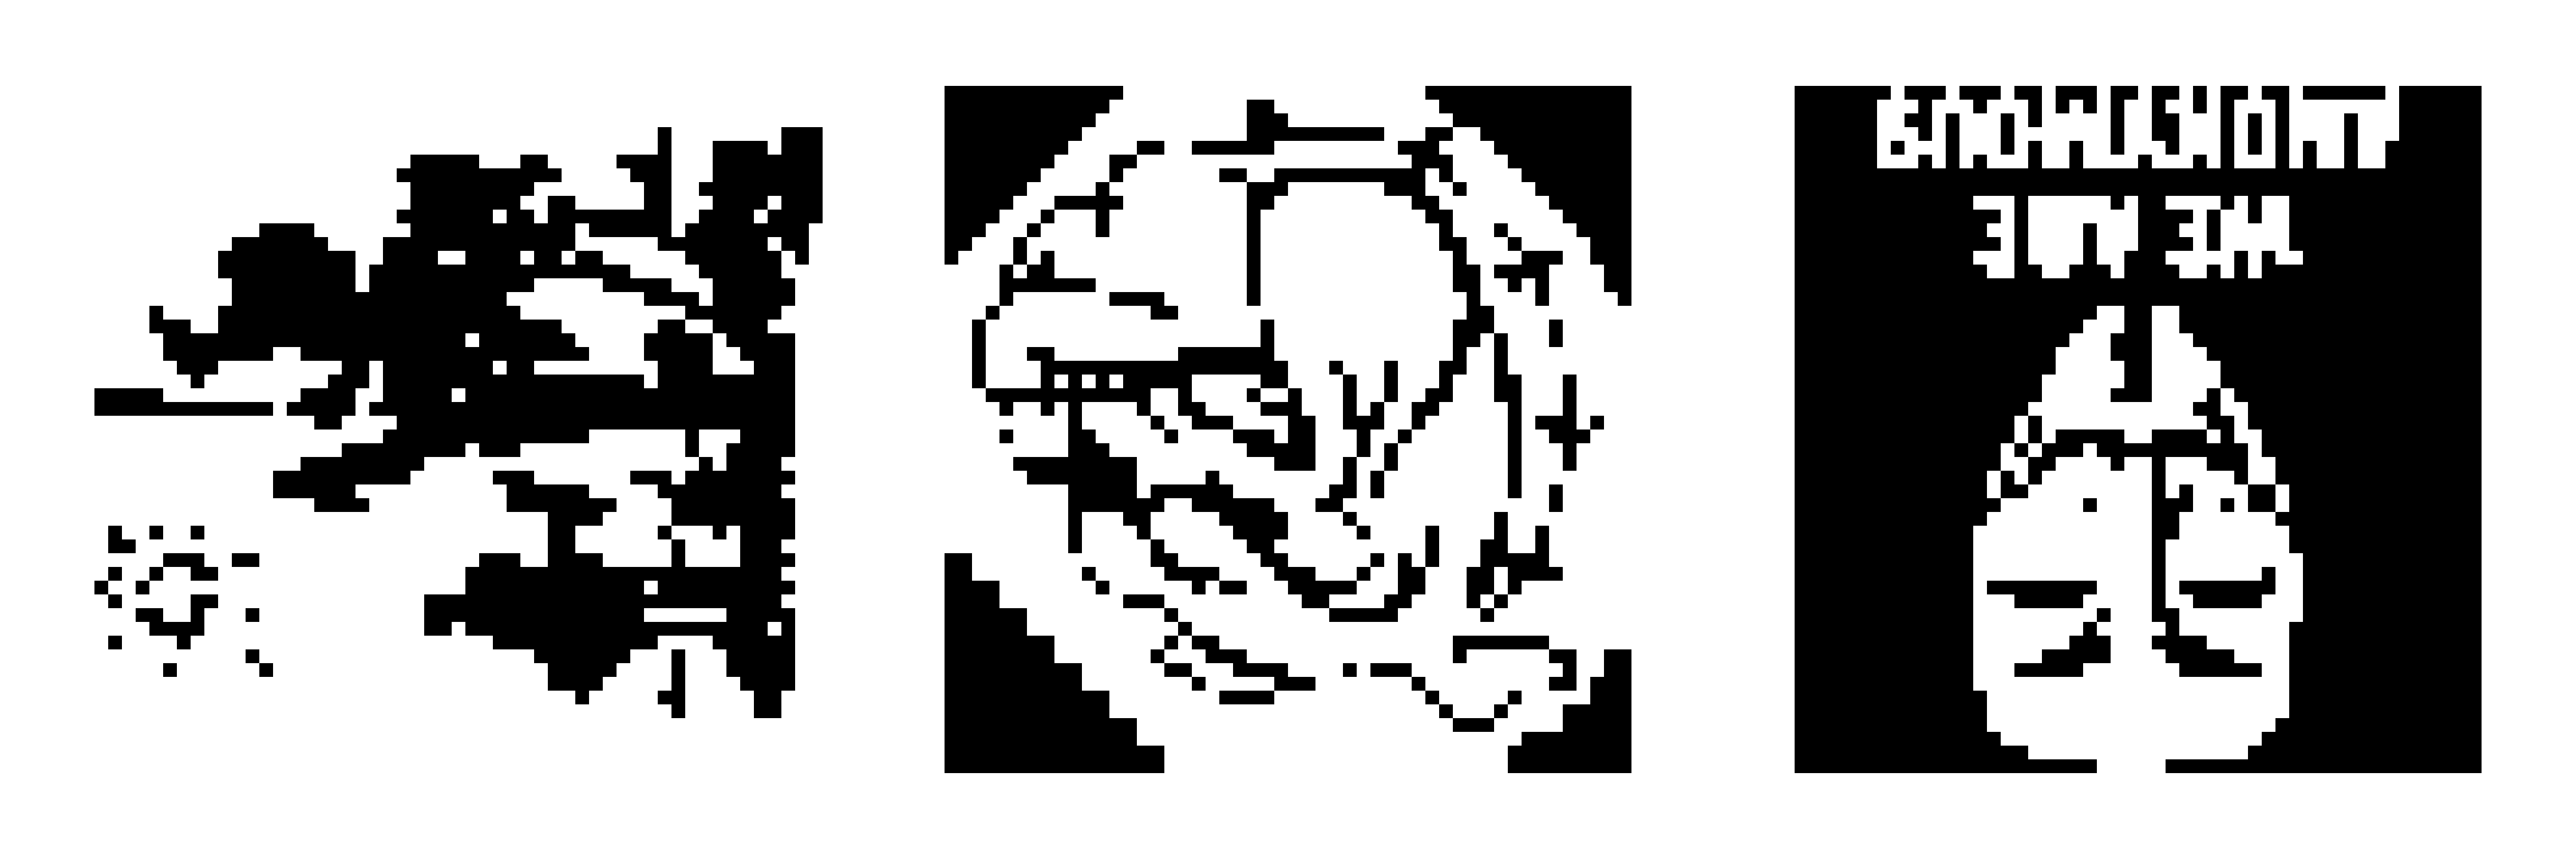
\includegraphics[width=0.5\textwidth]{imágenes/figura8.png}
    \caption{Imágenes rotadas $180^{\circ}$.}
    \label{fig:figura8}
\end{figure}

\begin{figure}[h]
    \centering
    \includegraphics[width=0.5\textwidth]{imágenes/figura9.png}
    \caption{Imágenes recuperadas.}
    \label{fig:figura9}
\end{figure}

\subsection{Existencia de estados epurios}
Un estado epurio es un estado estable que la red aprendió sin que se le enseñara. Para evaluar la existencia de estos estados, vamos a intentar recuperar patrones inversos y combinaciones lineales de una cantidad impar de imágenes del entrenamiento.

\begin{figure}[h]
    \centering
    \includegraphics[width=0.5\textwidth]{imágenes/figura10.png}
    \caption{Imágenes invertidas.}
    \label{fig:figura10}
\end{figure}

\begin{figure}[h]
    \centering
    \includegraphics[width=0.5\textwidth]{imágenes/figura11.png}
    \caption{Imágenes recuperadas.}
    \label{fig:figura11}
\end{figure}

\begin{figure}[h]
    \centering
    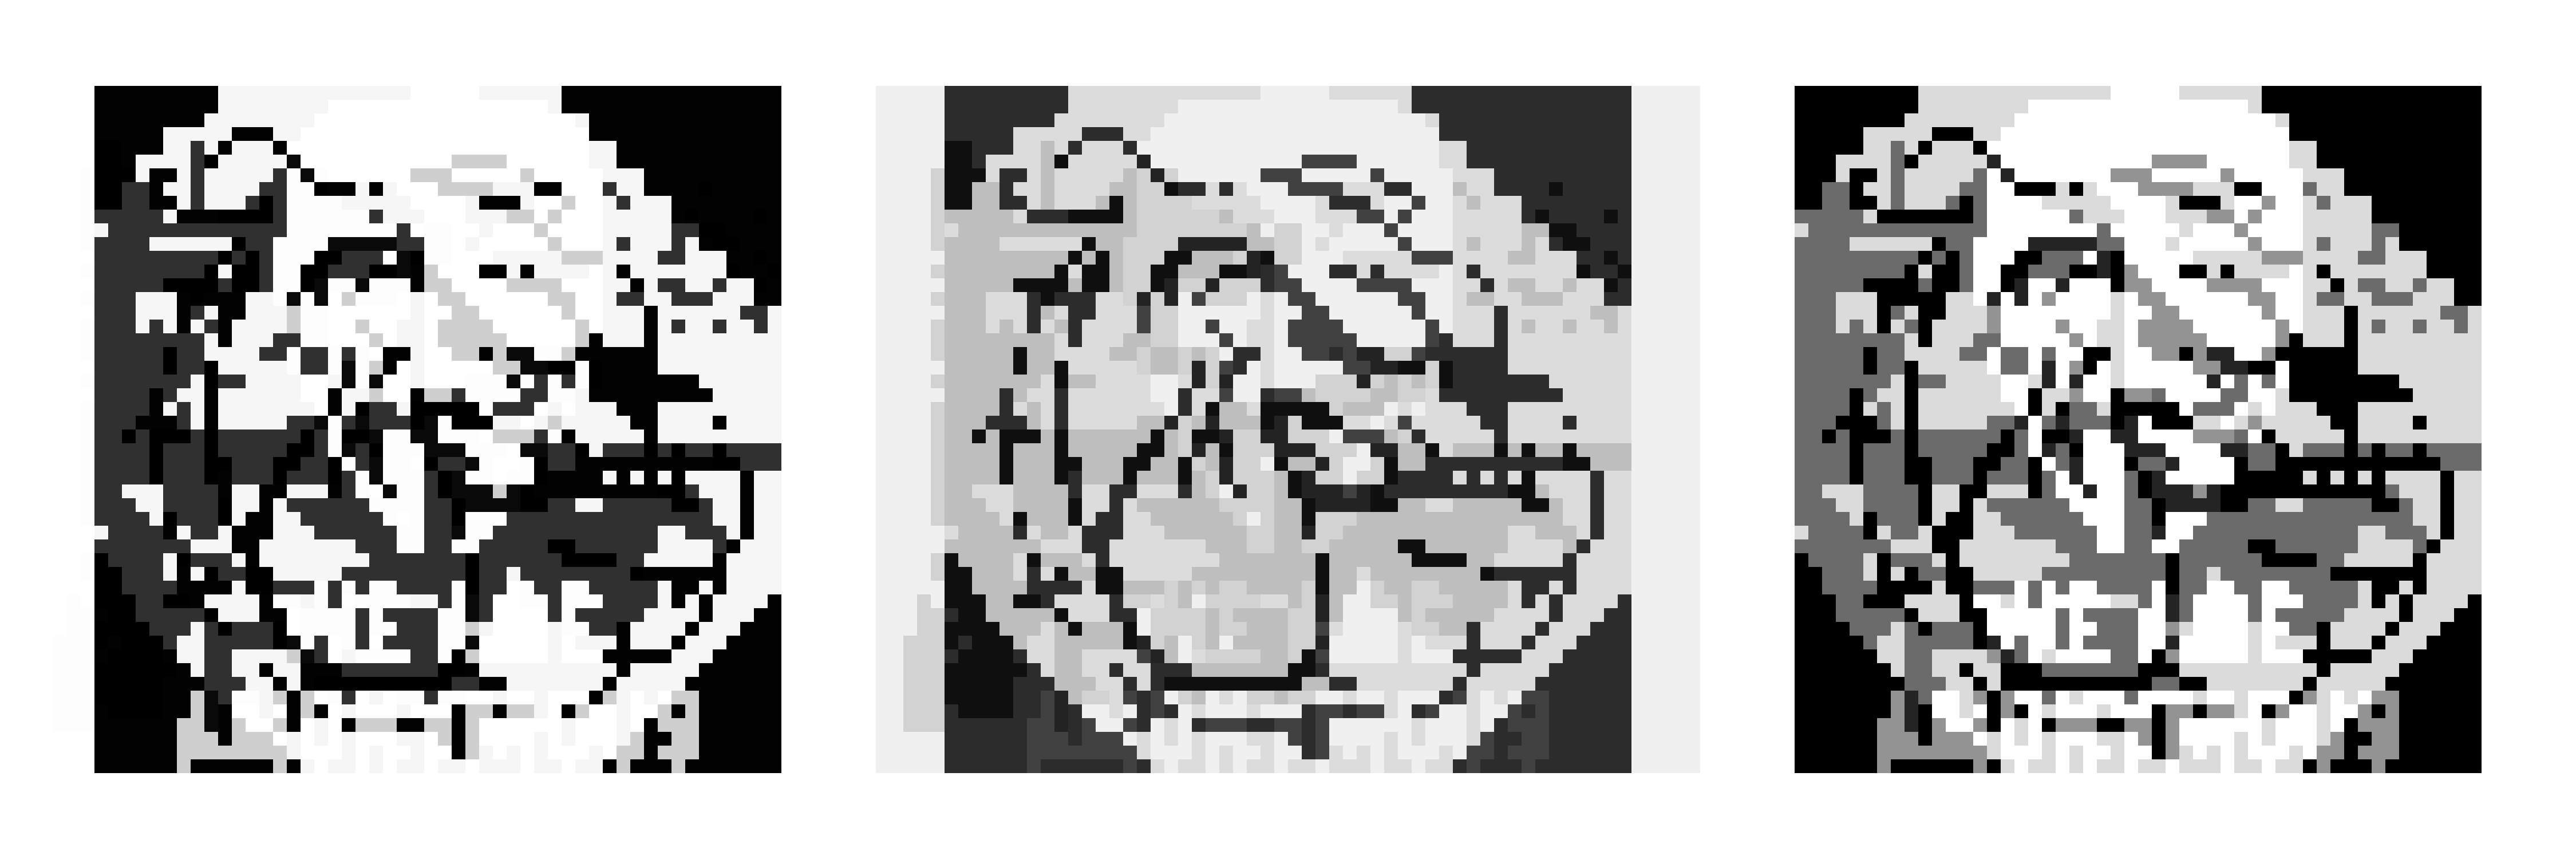
\includegraphics[width=0.5\textwidth]{imágenes/figura12.png}
    \caption{Imágenes combinadas linealmente.}
    \label{fig:figura12}
\end{figure}

\begin{figure}[h]
    \centering
    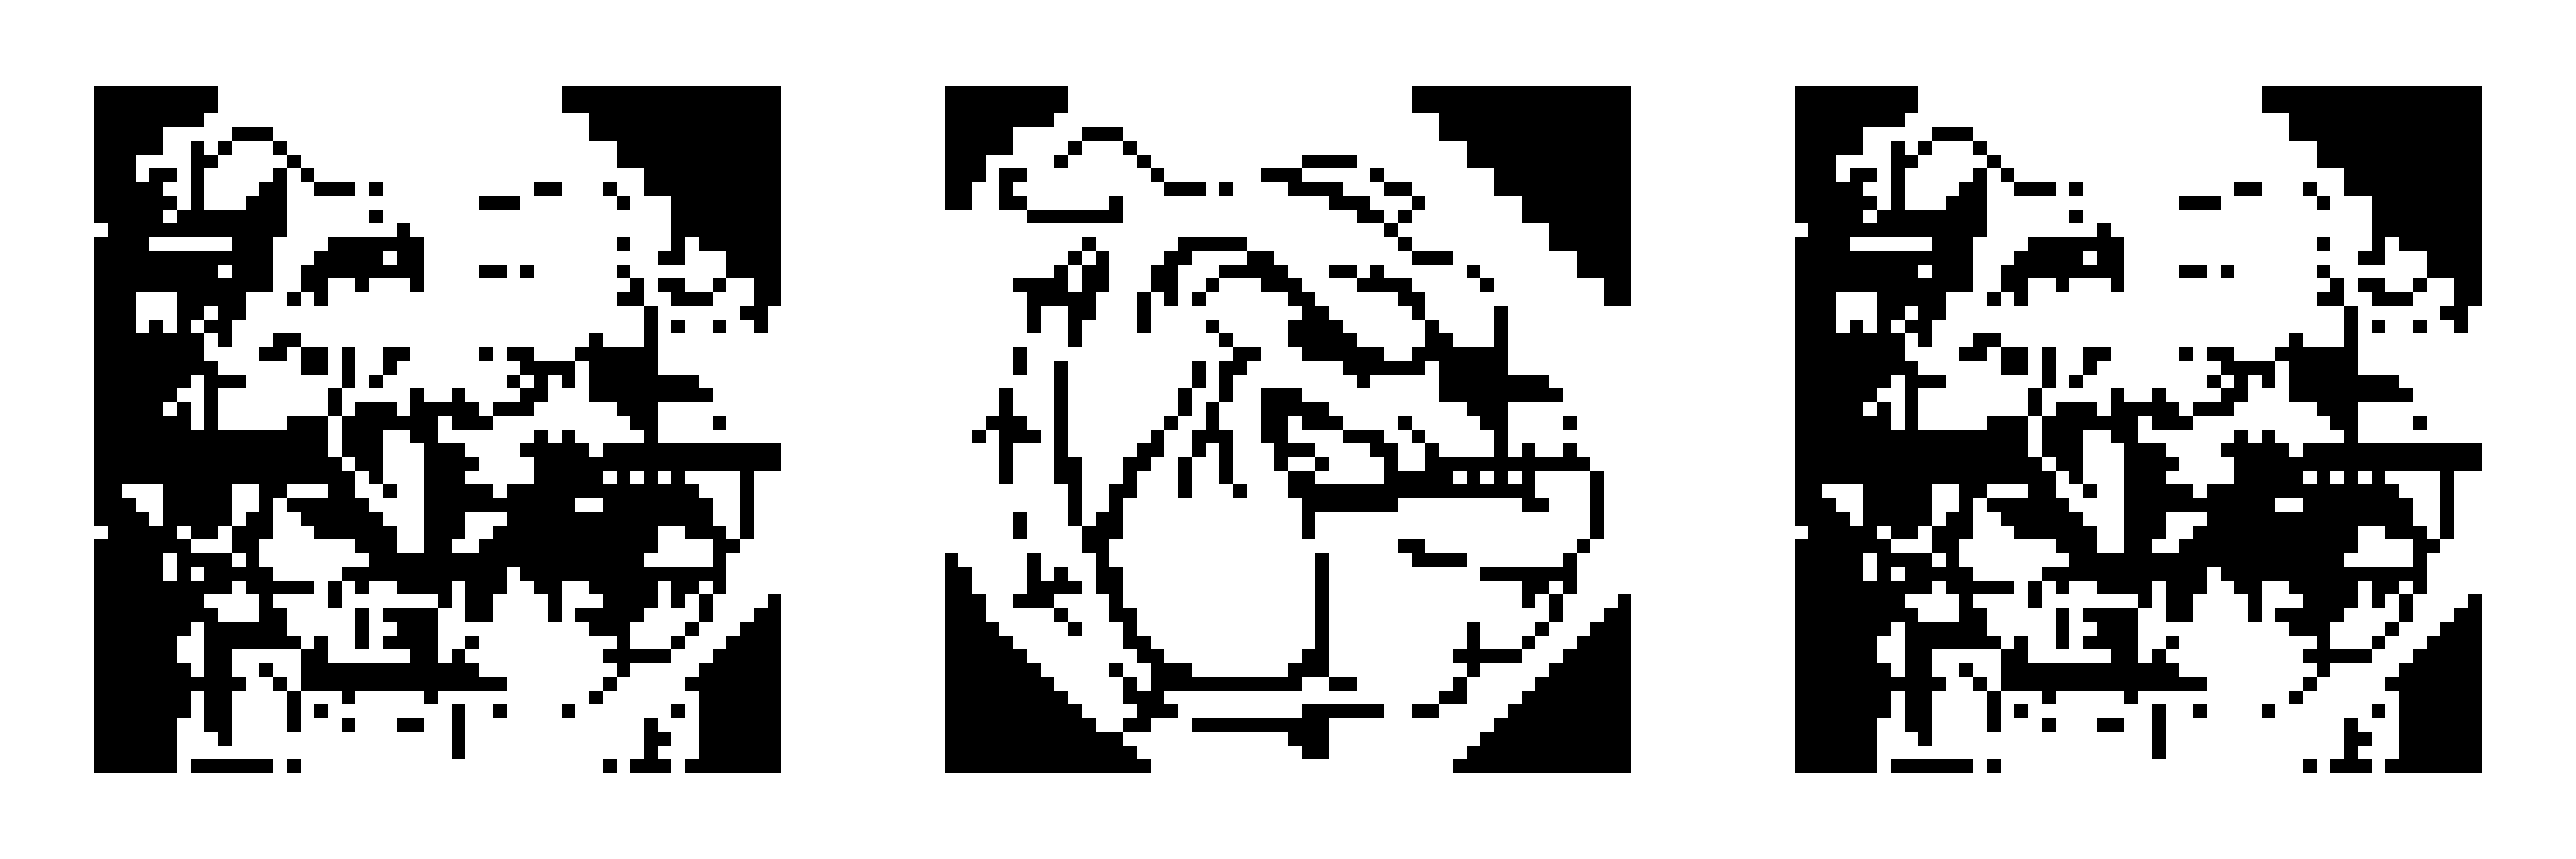
\includegraphics[width=0.5\textwidth]{imágenes/figura13.png}
    \caption{Imágenes recuperadas.}
    \label{fig:figura13}
\end{figure}

La red recupera estos estados estables, que no se le enseñaron. Y así se verifica la existencia de estados epurios.

\subsection{Entrenamiento con todas las imágenes}
Cuando entrenamos la red con las imágenes de la ~\ref{fig:figura1}, obtenemos al verificar su aprendizaje, es decir al intentar recuperar esas mismas imágenes, que la red no aprendió correctamente.

\begin{figure}[h]
    \centering
    \includegraphics[width=0.5\textwidth]{imágenes/figura14.png}
    \caption{Imágenes recuperadas.}
    \label{fig:figura14}
\end{figure}

La red no puede aprender bien los 6 patrones. Esto se debe a un punto débil de Hopfield: su capacidad de almacenamiento, que evidentemente, es excedida en este caso con 6 patrones.

\section{Capcaidad de la red}
\subsection{Capacidad máxima en función del tamaño y error aceptable}
En función del tamaño $N$ de la red buscamos, empíricamente, cuál es su máxima capacidad de almacenamiento $p_{\text{máx}}$ si toleramos cierta probabilidad de error $P_{\text{error}} = \frac{#\text{patrones recuperados}}{#\text{patrones totales}}$.
Para medir esto, simulamos un ciclo en el cual agregamos más patrones pseudo-aleatorios a medida que la red los aprende, tomando como prueba de que pudo con ellos, que $P_{\text{error}} sea menor a cierto número, es decir, que el cociente entre la cantidad de patrones recuperados y patrones totales sea menor a uno menos esa probabilidad tolerada $1 - P_{\text{error}}$.
Obtenemos entonces, para éste experimento, la siguiente tabla:

\begin{table}[h]
    \centering
    \begin{tabular}{|c|c|}
        \hline
        $P_{\text{error}}$ & $p_{\text{máx}} / N$ \\
        \hline
        0.001 & 0.1 \\
        \hline
        0.0036 & 0.13 \\
        \hline
        0.01 & 0.12 \\
        \hline
        0.05 & 0.2 \\
        \hline
        0.1 & 0.3 \\
        \hline
    \end{tabular}
    \caption{$p_{\text{máx}} / N$ para valores de $P_{\text{error}}$ determinados.}
    \label{tab:tabla1}
\end{table}

\subsection{Capacidad de la red con patrones correlacionados}
Ahora vamos a realizar el mismo experimento, sólo que esta vez, vamos a ir haciendo que la red aprenda más y más patrones correlacionados. Para eso partimos del patrón anterior y le agregamos ruido para crear uno nuevo.

\begin{table}[h]
    \centering
    \begin{tabular}{|c|c|}
        \hline
        $P_{\text{error}}$ & $p_{\text{máx}} / N$ \\
        \hline
        0.001 & 0.02 \\
        \hline
        0.0036 & 0.02 \\
        \hline
        0.01 & 0.02 \\
        \hline
        0.05 & 0.02 \\
        \hline
        0.1 & 0.02 \\
        \hline
    \end{tabular}
    \caption{$p_{\text{máx}} / N$ para valores de $P_{\text{error}}$ determinados, entrenando la red con patrones correlacionados entre sí.}
    \label{tab:tabla2}
\end{table}

Evidentemente la red no puede generalizar si se le enseñan patrones demasiado parecidos, no logra diferenciar entre mínimos locales superpuestos en la función de energía.

\begin{thebibliography}{9}

\bibitem{autor1}
John Hertz, Anders Krogh, Richard G. Palmer, \textit{Introduction to the Theory of Neural Computation}.

\end{thebibliography}

\end{document}